\section{Results}
In this study, we conducted an empirical investigation to evaluate the impact of interaction types(web v.s. chatbot) and correction formats(highlighting expert titles or not) on fact-checking effectiveness(RQ1), user intention to use(RQ2) and further analyzed which conditions help increase users' intention to check. 
For ease of description, we use \textbf{Interaction*Format} to denote our experimental conditions. 
"Interaction" can be classified as "web" and "chatbot", which refer to using the webpage or the chatbot to obtain fact-checking results, respectively.  
"Format" can be "Regular" or "Highlighted"(Highlighted expert titles).

We used the two-way ANOVA to examine the main effects and interactions.
Before that, a Shapiro-Wilk normality test was conducted to validate the normality assumption. The results showed that our data violated this assumption. 
Therefore, we used the Aligned Rank Transform(ART) procedure from the R-language Artool package to conduct the nonparametric factorial ANOVA.

\begin{table}[width=.9\linewidth,cols=5,pos=h]
    \caption{Descriptive Analysis of all measured dependent validate}\label{tbl1}
    \label{tab:descriptive}
    \begin{tabular*}{\tblwidth}{@{} LCCCC@{} }
    \toprule
    \textbf{Dependent}&\textbf{Web*Regualr}&\textbf{Web*Expert}&\textbf{Chatbot*Regualr} & \textbf{Chatbot*Expert}\\
    \textbf{variable}&(N=80)&(N=75)&(N=83)&(N=89)\\
     & Mean (SD) & Mean (SD) & Mean (SD) & Mean (SD) \\
    \midrule
    \textbf{Perceived Effectiveness}&\textbf{4.344 (0.638)} & 4.080 (0.760) & 4.165(0.735) & 4.322(0.585)\\
    \textbf{Objective Effectiveness}&1.538 (1.501) & 1.573 (1.454) & \textbf{1.807(1.224)} & 1.742(1.442)\\
    \textbf{Cognitive Effort}&3.900 (0.727) & 3.733 (0.786) & 4.169(0.664) & \textbf{4.174(0.743)}\\
    \textbf{Intention to Use}&3.987 (0.851) & 3.729 (0.838) & 3.948(0.688) & \textbf{3.993(0.680)}\\
    \textbf{Intention to Check}&4.069 (0.724) & 3.727 (0.807) & \textbf{4.102(0.688)} & 4.006(0.861)\\
    \bottomrule
    \end{tabular*}
    \end{table} 

    \begin{figure*}
        \centering
          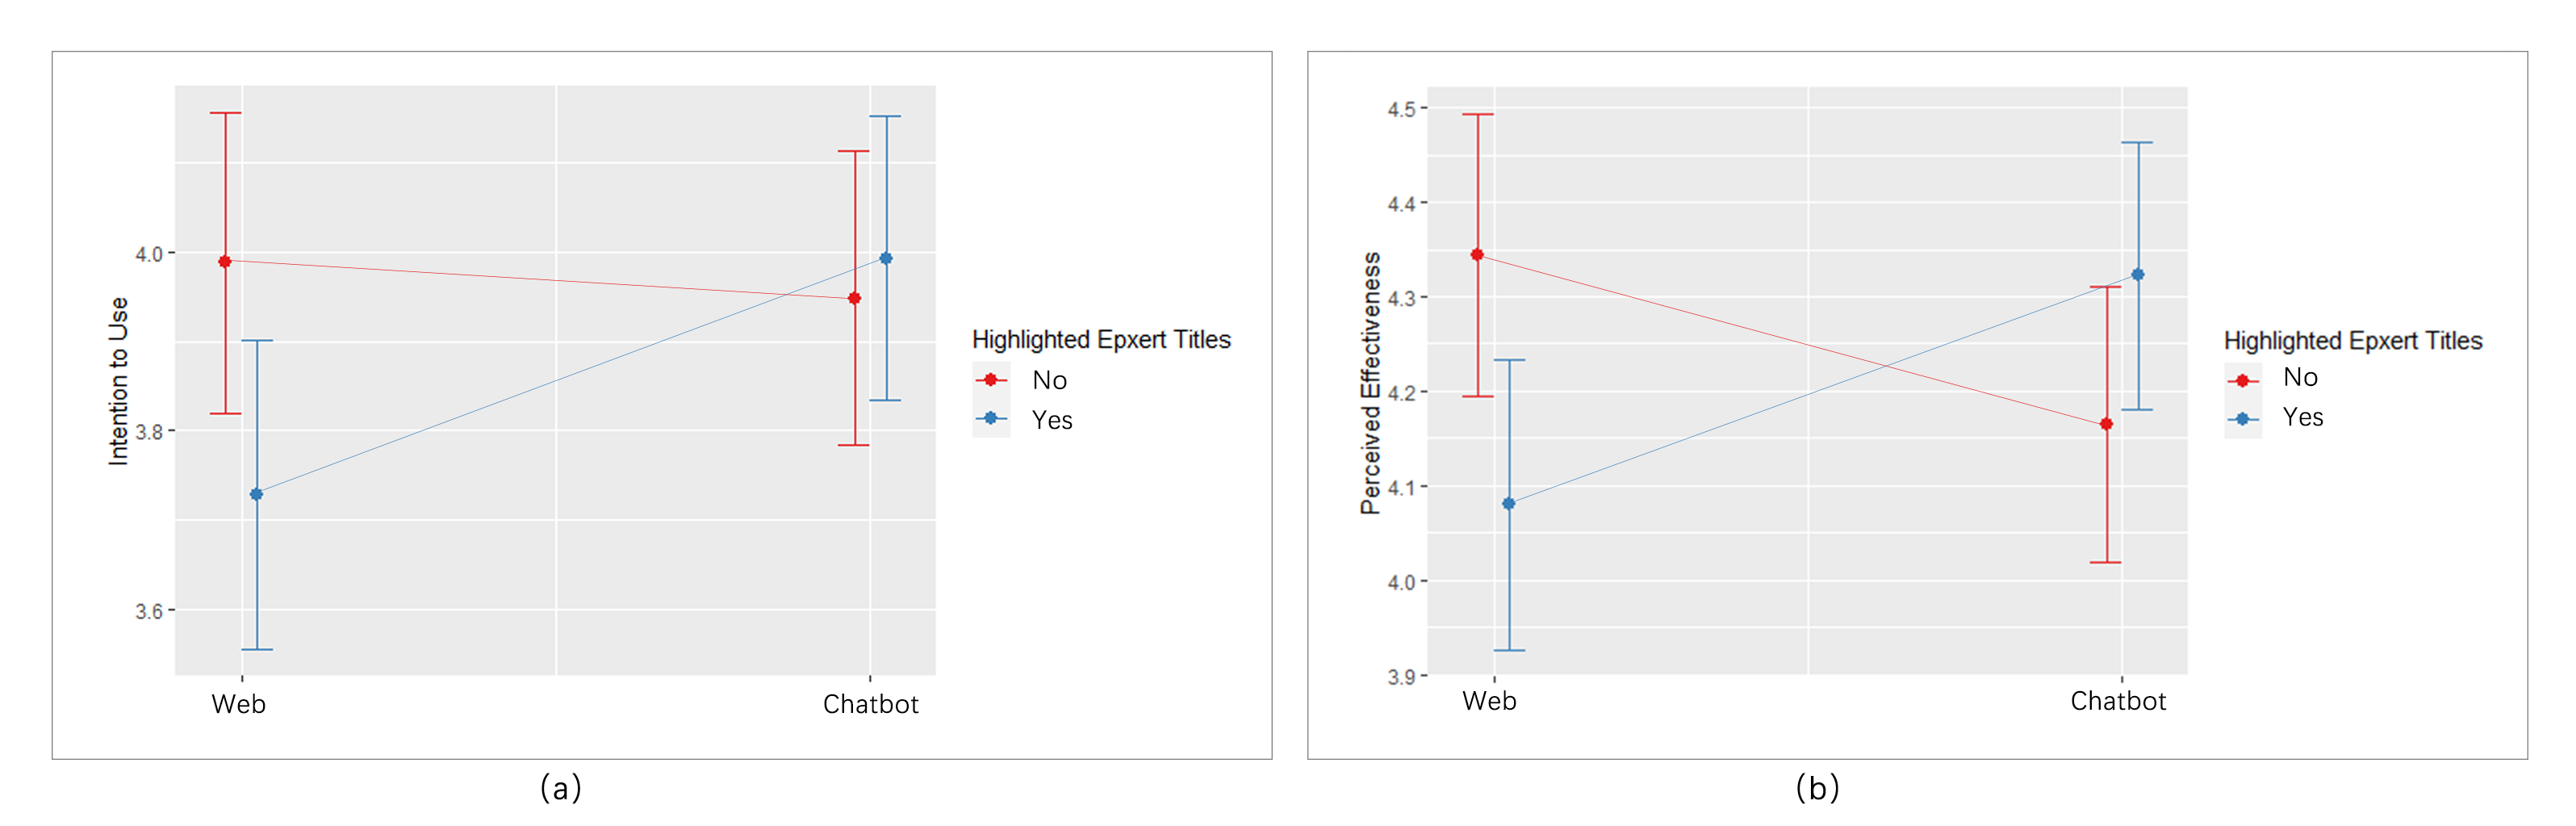
\includegraphics[width=\textwidth,height=2in]{figs/Interaction.png}
        \caption{Interaction effects between interaction type and currection format on a). perceived effectiveness and b). intention to use.}
        \label{FIG:interaction}
    \end{figure*}
    \begin{figure*}
        \centering
          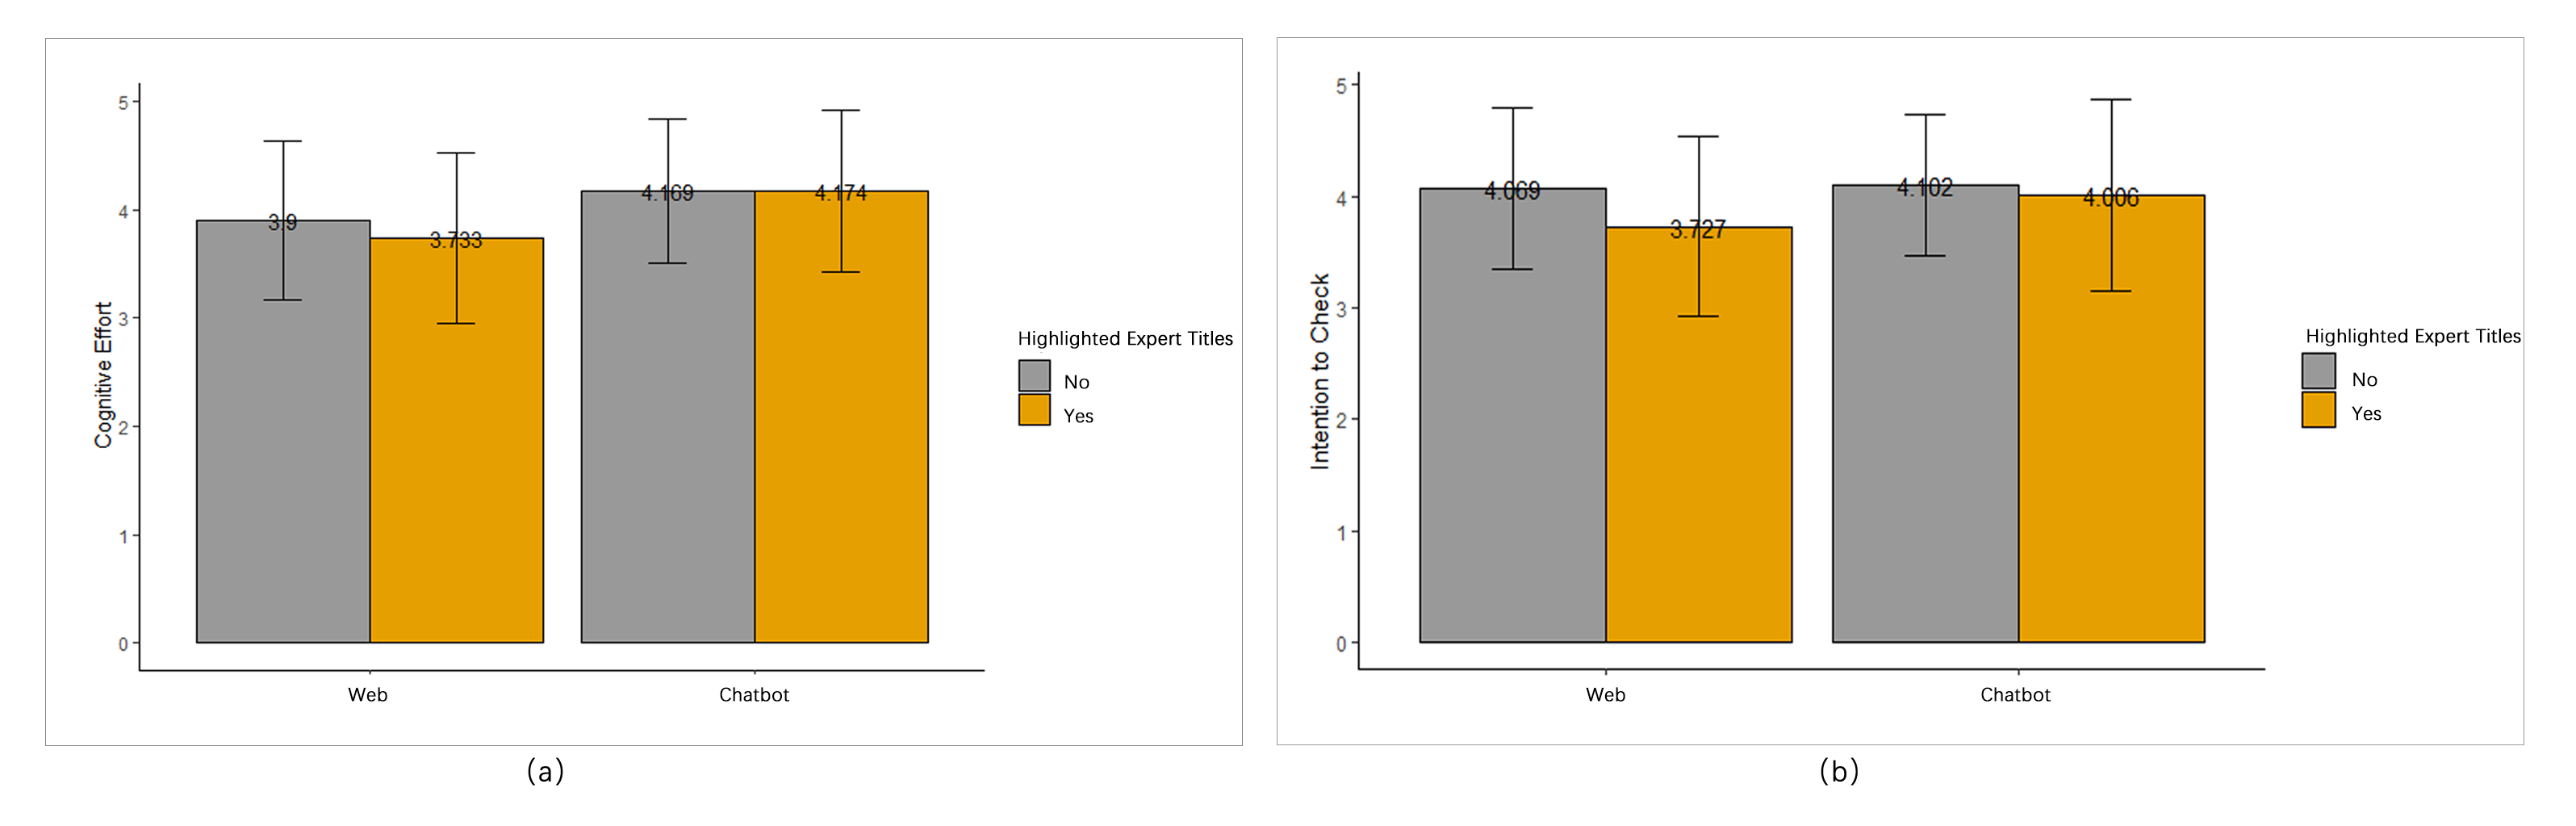
\includegraphics[width=\textwidth,height=2in]{figs/Maineffect.png}
        \caption{Main effects between interaction type and currection format on a). cognitive effect and b). intention to check.}
        \label{FIG:maineffect}
    \end{figure*}
\subsection{Evaluation of Currection Effectiveness}
To comprehensively measure the correction effectiveness, we evaluated the experimental conditions from both subjective and objective aspects.
The results revealed an interaction effect in subjective effectiveness, while there was no significant difference in objective effectiveness.

\subsubsection{Perceived Effectiveness}
The 2*2 ANOVA shows a significant interaction effect between interaction type and format on objective effectiveness, F(1, 323)=6.24, p<0.05, $\eta^{2}$=0.019.
We can observe that when participants use the web for fact-checking, the emphasis on expert titles decreases their perceived effectiveness.
However, there is an opposite trend when using the chatbot(see Figure~\ref{FIG:interaction}(a)).
Besides, the Chatbot*Highlighted design has a similar level of perceived effectiveness with the Web*Regualr(Table~\ref{tab:descriptive}).

\subsubsection{ Objectiveness Effectiveness}
\begin{table}
    \caption{Participants' accuracy on objective effectiveness questions}
    \label{tab:accuracy}
    \begin{tabular*}{\tblwidth}{@{} LCCC@{} }
     \toprule
     \textbf{Conditions} & Pre-test & Post-test & Improvement\\
     \midrule
     \textbf{Web * Regualr} & 30.2\% & 55.8\% & 25.6\% \\
     \textbf{Web * Highlighted} & 26.9\% & 53.1\% & 26.2\% \\ 
     \textbf{Chatbot * Regualr} & 25.3\% & 55.4\% & \textbf{30.12\%} \\
     \textbf{Chatbot * Highlighted} & 31.46\% & 60.5\% &29.0\%\\
     \bottomrule
    \end{tabular*}
  \end{table}

Figure~\ref{tab:accuracy} shows the participants' performance on the objective effectiveness questions in the pre-test and post-test. 
Participants answered the same questions in both tests, and we measured objective effectiveness by the improvement in their accuracy.
It can be seen that participants had better performance in the chatbot condition, while there was no significant effect on whether or not the expert title was highlighted.
In the web condition, participants' accuracy improved by 25.6\% and 26.2\% in the "Regular" and the "Highlighted" conditions, while in the chatbot condition, this accuracy was 30.1\% and 29.0\%, respectively.
The results of two-way ANOVA do not show any significant main effects or an interaction effect, indicating that there is no significant difference in the correction effect between these four experimental conditions.

\subsection{Evaluation of Users' Intention}
We examine the impact of the tool on user's behavioral tendencies from both their intention to use this tool and their intention to fact-check it in the future.
Before that we measured the cognitive effort of users in different experimental conditions.
As mentioned before, people are not willing to spend extra cognitive effort to verify the authenticity of information. If the design can help users reduce the cognitive effort, this may have a positive impact on their behavioral tendencies, which is the reason we measured this variable.
There, higher values of the variable indicate easier of use and less cognitive effort.

\subsubsection{Cognitive Effort}
Analysis of cognitive effort yields a significant main effect of interaction type, F(1, 323)=20.239, p < 0.001, $\eta^{2}$ = 0.059, indicating that participants expend less cognitive effort to check facts when using chatbots compared to using the web(see Figure~\ref{FIG:maineffect}(a)). 
The results do not show a significant main effect of format or an interaction effect.

\subsubsection{Intention to Use}
The main effects of interaction type and format are not found, but the interaction effect is significant, F (1, 323) = 5.310, p < 0.05, $\eta^{2}$ =0.022. 
Participants in the highlighted format reported lower intention to use than in the normal format condition when they use the web, but this effect disappears under the chatbot condition(see Figure~\ref{FIG:interaction}(b)).
There is no significant difference between the regular and highlighted formats when the chatbot is applied. Besides, the chatbot*highlighted design leads to the highest intention to use(Mean=3.993,SD=0.680).

\subsubsection{Intention to Check}
We also investigated participants' intention to conduct further fact-checks in the future.
We find significant main effects for interaction type(F(1, 323) = 4.202, p = 0.041, $\eta^{2}$=0.013) and coffection format (F(1, 323) = 5.453, p = 0.020, $\eta^{2}$ = 0.017).
Specifically, The chatbot design can increase users' intention to verify information, especially under the condition of highlighting expert titles.
However, emphasizing expert titles can somewhat reduce the intention to check(see Figure~\ref{FIG:maineffect}(b)).
